% TODO:
% --    Grafico con google sheets della soddisfazione media per ogni app?

Costruire un sistema avente come punto cardine l'usabilità risulta un progetto
estremamente ambizioso senza avere punti di riferimento, per questo è stato
valutato l'utilizzo di un discount usability test.  Sono state selezionate
diverse applicazioni e diversi soggetti uniformemente distribuiti lungo gli
scaglioni identificati al termine della fase precente.  Andiamo ad indicare
quindi i dettagli della fase di valutazione delle applicazioni esistenti.

\subsection{Metodologia di test}
La valutazione delle applicazioni esistenti è stata effettuata secondo due
modalità: una \emph{expert usability review} da noi effettuata e un
\emph{discount usability test}.  Rispetto a quest'ultimo si è utilizzata la
metodologia \emph{thinking aloud}, nella quale gli utenti sono stati invitati a
compiere svariati task descrivendo l'azione intrapresa.  Una volta completato il
task è stato richiesto ai partecipanti di dare una valutazione all'immediatezza
del task utilizzando una scala Likert con valori compresi fra 1 (per niente
intuitivo) e 5 (immediato).  Nel caso in cui il task sia risultato impossibile
si è attribuito il valore 0 alla propria facilità di completamento.
\subsubsection{Linee guida}
Per valutare l'usabilità delle applicazioni in esame si sono dapprima valutate
funzionalità principali tramite expert usability review.  In questa fase si è
cercato di valutare la facilità di navigazione, la completezza funzionale
dell'applicazione e alcune funzioni legate all'accessibilità. 
Oltre ad una descrizione informale dei punti di forza e delle debolezze delle applicazioni in esame,
si è poi proceduto a valutare (in fig. \ref{fig:valutazionelineeguida}),la facilità di navigazione, la ricchezza
di contenuti, la presenza di aspetti social e la facilità di scoperta di nuove ricette nelle app.
A tale fine si è utilizzata una scala compresa fra 1 e 5 dove 1 indica un punto di debolezza, mentre
5 indica un aspetto ben implementato.\\
\begin{figure}[H]
 \centering
 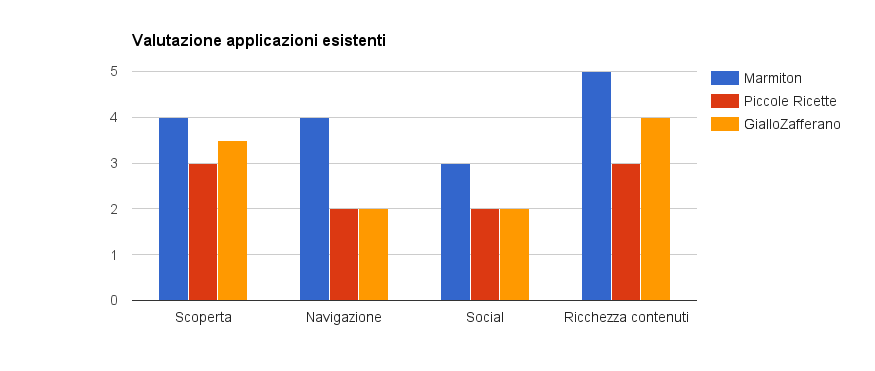
\includegraphics[width=\textwidth]{img/valutazionelineeguida}
 \label{fig:valutazionelineeguida}
\end{figure}
Durante la fase
di \emph{user testing} si è privilegiata invece un'analisi focalizzata su task
fondamentali del dominio in esame.  In questa maniera è possibile ottenere
indicazioni sull'utilizzo ordinario delle applicazioni e sulle loro
funzionalità.  L'unica eccezione a questo approccio riguarda una funzionalità di
accessibilità quale la possibilità di modificare la dimensione del testo.\\
Si riporta in seguito la lista dei task selezionati:
\begin{enumerate}
	\item Cercare una ricetta da noi precedentemente individuata;
	\item Aggiungere una ricetta ai preferiti;
	\item Aggiungere gli ingredienti di una ricetta alla lista della spesa;
	\item Cercare ricette appartenenti ad una determinata categoria
		(vegetariane);
	\item Condividere una ricetta tramite social network;
	\item Creare un menù per la cena o per il pranzo, composto da tre portate;
	\item Cercare istruzioni video relative ad una ricetta;
	\item Cercare commenti relativi ad una ricetta;
	\item Inserire un commento personale riguardo ad una ricetta;
	\item Effettuare la spesa, spuntando uno ad uno gli alimenti;
	\item Cercare un abbinamento per una ricetta specifica;
	\item Cercare ricette nuove proposte dall'applicazione;
	\item Cambiare la dimensione del testo.
\end{enumerate}

\subsection{Applicazioni utilizzate per il test comparativo}
Sono state selezionate tre applicazioni mobili disponibili sui principali market
e testate utilizzando il sistema operativo Android.  Si riporta la lista delle
suddette applicazioni:
\begin{itemize}
	\item Piccole ricette\cite{PiccoleRicette}, piccola applicazione avente una base d'utenza
	limitata e un numero rilevante di ricette (circa 1800).
\item GialloZafferano\cite{GialloZafferano}, applicazione mobile dai gestori dell'omonimo
	sito, popolare e con base di ricette notevole (circa 3400).
\item Marmiton\cite{Marmiton}, applicazione francese con una grande base d'utenza e
	un massiccio numero di ricette disponibili (circa 64.000).
\end{itemize}

\subsection{Piccole Ricette}
È stata utilizzata la versione gratuita del programma contenente pubblicità
all'avvio in forma di video, che risulta essere molto intrusiva.  La navigazione
dell'applicazione non è immediata, in quanto ad esempio il menù laterale viene
utilizzato soltanto per accedere alle impostazioni e viola concetti fondamentali
di usabilità quali coerenza esterna in quanto, solitamente,
i menù laterali vengono utilizzati dalle applicazioni come menu di navigazione.
La lista della spesa non presenta checkbox e non rende chiara la cliccabilità
dei vari elementi, non presentando inviti o aiuti per gli utenti.  La ricerca
risulta essere molto espressiva.  Nei risultati della ricerca, invece, le
ricette sono descritti tramite simboli il cui significato non è chiaro.
Non è ben descritto il senso di progressione tra i vari passi della ricetta.

\subsection{GialloZafferano}
Anche in questo caso è stata utilizzata la versione gratuita dell'applicazione.
Quest'ultima per effettuare operazioni sulle singole ricette utilizza un menù
contestuale attivato dal simbolo "+" e contenente un semicerchio di icone.
Queste ultime risultano essere poco chiare non avendo legenda o descrizione
testuale oltre ad essere numerose e complesse.  Per quanto riguarda le
istruzioni in forma di video per le ricette una volta attivati essi non
rimangono in primo piano e non è immediato comprendere come interromperne la
riproduzione.  È presente una modalità per la condivisione tramite mail che non
risulta però essere chiara ed utilizzabile.  L'applicazione non rende chiaro
all'utente il senso di progresso durante la preparazione di una ricetta.
Riguardo all'accessibilità l'applicazione presenta un'impostazione per
modificare la grandezza del testo, la quale utilizza uno slider il cui
indicatore è colorato con le restanti parti dello stesso colore dello sfondo.
Questo rende complicato comprendere l'interazione possibile con tale widget.

\subsection{Marmiton}
Nonostante si tratti di un'applicazione in lingua francese, sia dall'expert
usability review, sia negli user test presentati in seguito, Marmiton è
risultata essere l'applicazione più apprezzata.  Essa è ricca di funzionalità e
contiene il database di ricette più esteso fra quelli considerati.  Permette
inoltre diverse modalità di \emph{discoverability} delle ricette, proponendo
selezioni tematiche (es. ricette natalizie, grandi classici, ricette del giorno)
e un'interessante modalità per ottenere una ricetta casuale tramite lo
squotimento del telefono.  La principale critica che è possibile muovere a tale
applicazione riguarda il menù laterale, che risulta leggermente prolisso. Un
altro problema riguarda la separazione tra video e le ricette stesse.  Nella
pagina delle singole ricette vengono infatti presentati dei video correlati che
non hanno nulla a che vedere con la ricetta, che causano qualche confusione.
L'applicazione, infine, presenta le migliori funzionalità sociali, potendo
condividere con la rete sociale le foto delle ricette appena preparate e
permettendo di sapere quante persone hanno aggiunto una ricetta ai propri
preferiti.



\subsection{Task e risultati dei test}
Si riportano quindi le soddisfazioni indicate dagli utenti
per i task descritti in precedenza relative ad ogni applicazione in esame:

\subsubsection{Cercare una ricetta}
\begin{tabular}{l c}
Piccole Ricette: & 3,5\\
GialloZafferano: & 4,5\\
Marmiton: & 4,3\\
\end{tabular}

\subsubsection{Aggiungere una ricetta ai preferiti}
\begin{tabular}{l c}
Piccole Ricette: & 2,8\\
GialloZafferano: & 3,3\\
Marmiton: & 4,1\\
\end{tabular}

\subsubsection{Aggiungere una ricetta alla lista della spesa}
\begin{tabular}{l c}
Piccole Ricette: & 3,3\\
GialloZafferano: & 3\\
Marmiton: & 4,4\\
\end{tabular}

\subsubsection{Cercare ricette che non presentino uno specifico ingrediente o di
una determinata classe}
\begin{tabular}{l c}
Piccole Ricette: & 3\\
GialloZafferano: & 3,3\\
Marmiton: & 2,7\\
\end{tabular}

\subsubsection{Condividere una ricetta}
\begin{tabular}{l c}
Piccole Ricette: & 4,3\\
GialloZafferano: & 4\\
Marmiton: & 4,3\\
\end{tabular}

\subsubsection{Creare un menù}
\begin{tabular}{l c}
Piccole Ricette: & 3,5\\
GialloZafferano: & 2,6\\
Marmiton: & 3,7\\
\end{tabular}

\subsubsection{Cercare istruzioni video}
\begin{tabular}{l c}
Piccole Ricette: & 3,2\\
GialloZafferano: & 2,8\\
Marmiton: & 2,6\\
\end{tabular}

\subsubsection{Cercare commenti}
\begin{tabular}{l c}
Piccole Ricette: & 4,5\\
GialloZafferano: & 5\\
Marmiton: & 4,3\\
\end{tabular}

\subsubsection{Inserire un commento personali}
\begin{tabular}{l c}
Piccole Ricette: & 4,6\\
GialloZafferano: & 4,3\\
Marmiton: & 4,3\\
\end{tabular}

\subsubsection{Effettuare la spesa}
\begin{tabular}{l c}
Piccole Ricette: & 4\\
GialloZafferano: & 3\\
Marmiton: & 3,6\\
\end{tabular}

\subsubsection{Cercare abbinamenti suggeriti}
\begin{tabular}{l c}
Piccole Ricette: & 0\\
GialloZafferano: & 0,5\\
Marmiton: & 1,3\\
\end{tabular}

\subsubsection{Cercare ricette nuove proposte}
\begin{tabular}{l c}
Piccole Ricette: & 3,6\\
GialloZafferano: & 4,5\\
Marmiton: & 4,6\\
\end{tabular}

\subsubsection{Cambiare dimensioni del testo}
\begin{tabular}{l c}
Piccole Ricette: & 0\\
GialloZafferano: & 3\\
Marmiton: & 0\\
\end{tabular}
